\documentclass[conference]{IEEEtran}
\usepackage{amsmath,amssymb}
\usepackage{booktabs}
\usepackage{graphicx}
\usepackage{microtype}
\usepackage{xcolor}
\usepackage{url}
\usepackage{multirow}

\title{Benchmarking Neural Surrogates for Hydrofoil RANS Flow,\\
Cavitation-Risk Prediction, and Hydrodynamic Shape Optimization}

\author{\IEEEauthorblockN{Anonymous Author(s)}
\IEEEauthorblockA{Affiliation withheld for review\\
Email withheld for review}}

\begin{document}
\maketitle

\begin{abstract}
We benchmark four neural surrogates for hydrofoil RANS prediction and design:
CNN-U-Net, a supervised physics-regularized point network, a Fourier neural
operator (FNO), and DeepONet. The dataset contains 381 valid OpenFOAM cases. Its
64-case validation set consists entirely of two NACA families that are absent
from training. The models predict flow fields, force coefficients, and
pressure-based cavitation risk. The physics-regularized network gives the best
pressure result ($R^2=0.966$) and cavitation-risk F1 score (0.921). DeepONet
gives the best lift and drag results ($R^2=0.996$ and $0.988$). Inference is
917--1801 times faster than OpenFOAM. We also use each surrogate for continuous
NACA shape optimization and rerun its best design in OpenFOAM. The resulting
lift-to-drag improvements range from 2.3\% to 79.7\% relative to the starting
foils. This end-to-end benchmark compares accuracy, speed, and the quality of
the final CFD-validated designs.
\end{abstract}

\begin{IEEEkeywords}
AI for science, CFD surrogate, neural operator, physics-informed learning, hydrofoil optimization, cavitation inception
\end{IEEEkeywords}

\section{Introduction}
Computational fluid dynamics (CFD) is widely used for hydrofoil analysis and
design. The difficulty is cost: optimization and operating sweeps may require
hundreds or thousands of Reynolds-averaged Navier--Stokes (RANS) solutions.
Neural surrogates reduce that repeated cost and are increasingly useful in
data-driven fluid mechanics \cite{brunton2020machine}. Their value should be
measured beyond field error. A model must also preserve forces, identify
low-pressure regions, and guide an optimizer toward a design that remains good
when it is returned to CFD.

CNN-U-Net, FNO, DeepONet, and physics-regularized networks represent the flow
map in different ways \cite{ronneberger2015unet,li2021fno,lu2021deeponet,raissi2019pinn}.
That makes them a useful benchmark set. Prior work often compares field metrics
alone. We extend the comparison to pressure, lift, drag, cavitation-risk
classification, runtime, and hydrodynamic shape optimization.

Earlier airfoil surrogates used convolutional or hybrid networks to predict
steady flow fields from geometry and operating conditions
\cite{guo2016steady,bhatnagar2019aerodynamic,sekar2019airfoils,thuerey2020rans}.
Physics-informed neural operators provide another route for combining PDE
structure with operator learning \cite{li2024pino}. Our study instead holds the
data and downstream optimizer fixed to compare four model families directly.

Twelve NACA four-digit families, eight angles of attack, and four Reynolds
numbers yield 384 OpenFOAM cases. After a force-coefficient quality check, 381
cases remain. The validation set contains every case from NACA 0015 and 2412,
so it measures generalization to geometries not used for training. All four
models use the same targets and split. Each model is then placed in the same
optimizer, and its selected design is independently rerun in OpenFOAM.

The contributions are:
\begin{itemize}
    \item a four-model benchmark on an unseen-geometry validation set, covering
    flow fields, force coefficients, runtime, and cavitation-risk screening;
    \item a common hydrodynamic shape-optimization experiment for all four
    surrogates; and
    \item an independent OpenFOAM rerun of each model's selected design.
\end{itemize}

Here, ``cavitation risk'' means pressure-threshold inception risk computed from
$C_p$. It is useful for screening low-pressure regions. It is not a multiphase
prediction of cavity length or shedding.

\section{Data and CFD Reference}
\subsection{Design space}
The dataset contains NACA 0006, 0008, 0010, 0012, 0015, 0018, 2412, 2415, 4412, 4415, 4418, and 4421 profiles generated from the standard four-digit parameterization \cite{abbott1959airfoils}. For each profile, we simulate angles of attack $\alpha\in\{-4,-2,0,2,4,6,8,10\}^{\circ}$ and Reynolds numbers $Re\in\{10^5,2\times10^5,5\times10^5,10^6\}$. The chord is 1~m, water density is 997~kg/m$^3$, and kinematic viscosity is $10^{-6}$~m$^2$/s, so the freestream speed is set by $U_\infty=Re\nu/c$. The far-field absolute pressure and vapor pressure are 101325 and 2300~Pa.

Each case is solved with OpenFOAM \texttt{simpleFoam} \cite{weller1998tensorial}, using steady incompressible RANS and the $k$--$\omega$ SST closure \cite{menter1994sst}. Angled freestream velocity is imposed at the inlet and far boundary. The solver runs for 300 iterations, and OpenFOAM's \texttt{forceCoeffs} provides total lift and drag references. Cell-centered fields are interpolated to a common $128\times64$ Cartesian grid over $x/c\in[-1,2]$ and $y/c\in[-0.75,0.75]$. Inputs include coordinates, operating parameters, three NACA geometry descriptors, a fluid mask, and signed distance to the profile.

An audit found no pressure fields duplicated across angle of attack and found
force files for all 384 cases. Three cases produced $|C_L|$ or $|C_D|>5$ and
were removed before splitting. This leaves 381 cases. All 64 cases from NACA
0015 and NACA 2412 form the unseen-geometry validation set. The remaining 317
cases train the models. No validation geometry therefore appears in training at
another operating condition.

\subsection{Targets and cavitation-risk definition}
The common output vector contains $U_x$, $U_y$, absolute pressure $p$, eddy viscosity, $k$, $\omega$, $C_p$, cavitation margin, $C_L$, and $C_D$. Grid fields use masked normalized mean-squared error, while the case-level force targets use normalized mean-squared error. OpenFOAM's kinematic gauge pressure $p_k$ is converted to absolute pressure as
\begin{equation}
 p=p_\infty+\rho p_k, \qquad C_p=\frac{p-p_\infty}{\tfrac{1}{2}\rho U_\infty^2}.
\end{equation}
For an ambient-pressure value $p_a$, the pressure-based inception margin is
\begin{equation}
 M(x,y;p_a)=p_a+C_p(x,y)\tfrac{1}{2}\rho U_\infty^2-p_v.
\end{equation}
A cell is labeled at risk when $M<0$. We evaluate this label at $p_a\in\{2500,3000,5000,10000,25000,101325\}$~Pa. This sweep creates a useful classification test from the predicted $C_p$ field without representing multiphase physics.

\section{Surrogates and Optimization}
\subsection{Model families}
The \textbf{CNN-U-Net} has three encoder/decoder levels, skip connections,
group normalization, GELU activations, and base width 16. It maps the complete
input grid to the output grid \cite{ronneberger2015unet}. The \textbf{FNO} has width 32, four operator
blocks, and 12 retained Fourier modes in each direction. One block is
\begin{equation}
h_{\ell+1}=\sigma\!\left(W_\ell h_\ell+
\mathcal{F}^{-1}\!\left(R_\ell\mathcal{F}(h_\ell)\right)\right).
\end{equation}
following the spectral operator construction of \cite{li2021fno}.
Here, $W_\ell$ is a local linear map and $R_\ell$ acts on the retained spectral
modes. The \textbf{DeepONet} uses three-layer, width-64 branch and trunk
networks with 64 basis functions. For output $k$,
\begin{equation}
\widehat{y}_k(\mathbf{x};\boldsymbol{\mu})=
\frac{\mathbf{b}_k(\boldsymbol{\mu})^\top\mathbf{t}_k(\mathbf{x})}{\sqrt{64}}+c_k,
\end{equation}
as in the branch--trunk construction of \cite{lu2021deeponet},
where $\boldsymbol{\mu}$ contains the operating and geometry parameters.

The \textbf{physics-regularized MLP} has three tanh layers of width 64. It is
supervised by CFD values at 1,024 sampled points per case. Its extra loss uses
the directional residuals
\begin{equation}
r_c=u_x+v_y,\quad r_x=u u_x+p_x/\rho,\quad r_y=v v_y+p_y/\rho,
\end{equation}
with $\mathcal{L}=\mathcal{L}_{\rm sup}+10^{-4}\mathcal{L}_{\rm phys}$,
following the residual-loss principle in \cite{raissi2019pinn}.
This is a lightweight physics regularizer, not a data-free PINN or a complete
RANS residual.

All models use AdamW with learning rate $2\times10^{-3}$, weight decay
$10^{-4}$, at most 120 epochs, patience 20, gradient clipping, and seed 7.
Normalization is computed from training cases only. The best checkpoint is
selected by validation loss. Model size ranges from 9,930 to 595,914 parameters
(Table~\ref{tab:performance}).

Figure~\ref{fig:training} reports the complete optimization histories rather
than only the selected checkpoints. Because the architectures consume the data
in different forms and the objective aggregates heterogeneous normalized
targets, loss magnitude should be interpreted within a model, not as a direct
cross-model accuracy metric. DeepONet reaches its minimum validation objective
at epoch 6, the physics-regularized network at epoch 30, FNO at epoch 54, and
CNN-U-Net at epoch 120. The isolated FNO spikes are retained in the record and
motivate reporting best-checkpoint results alongside the full history.

\begin{figure*}[t]
\centering
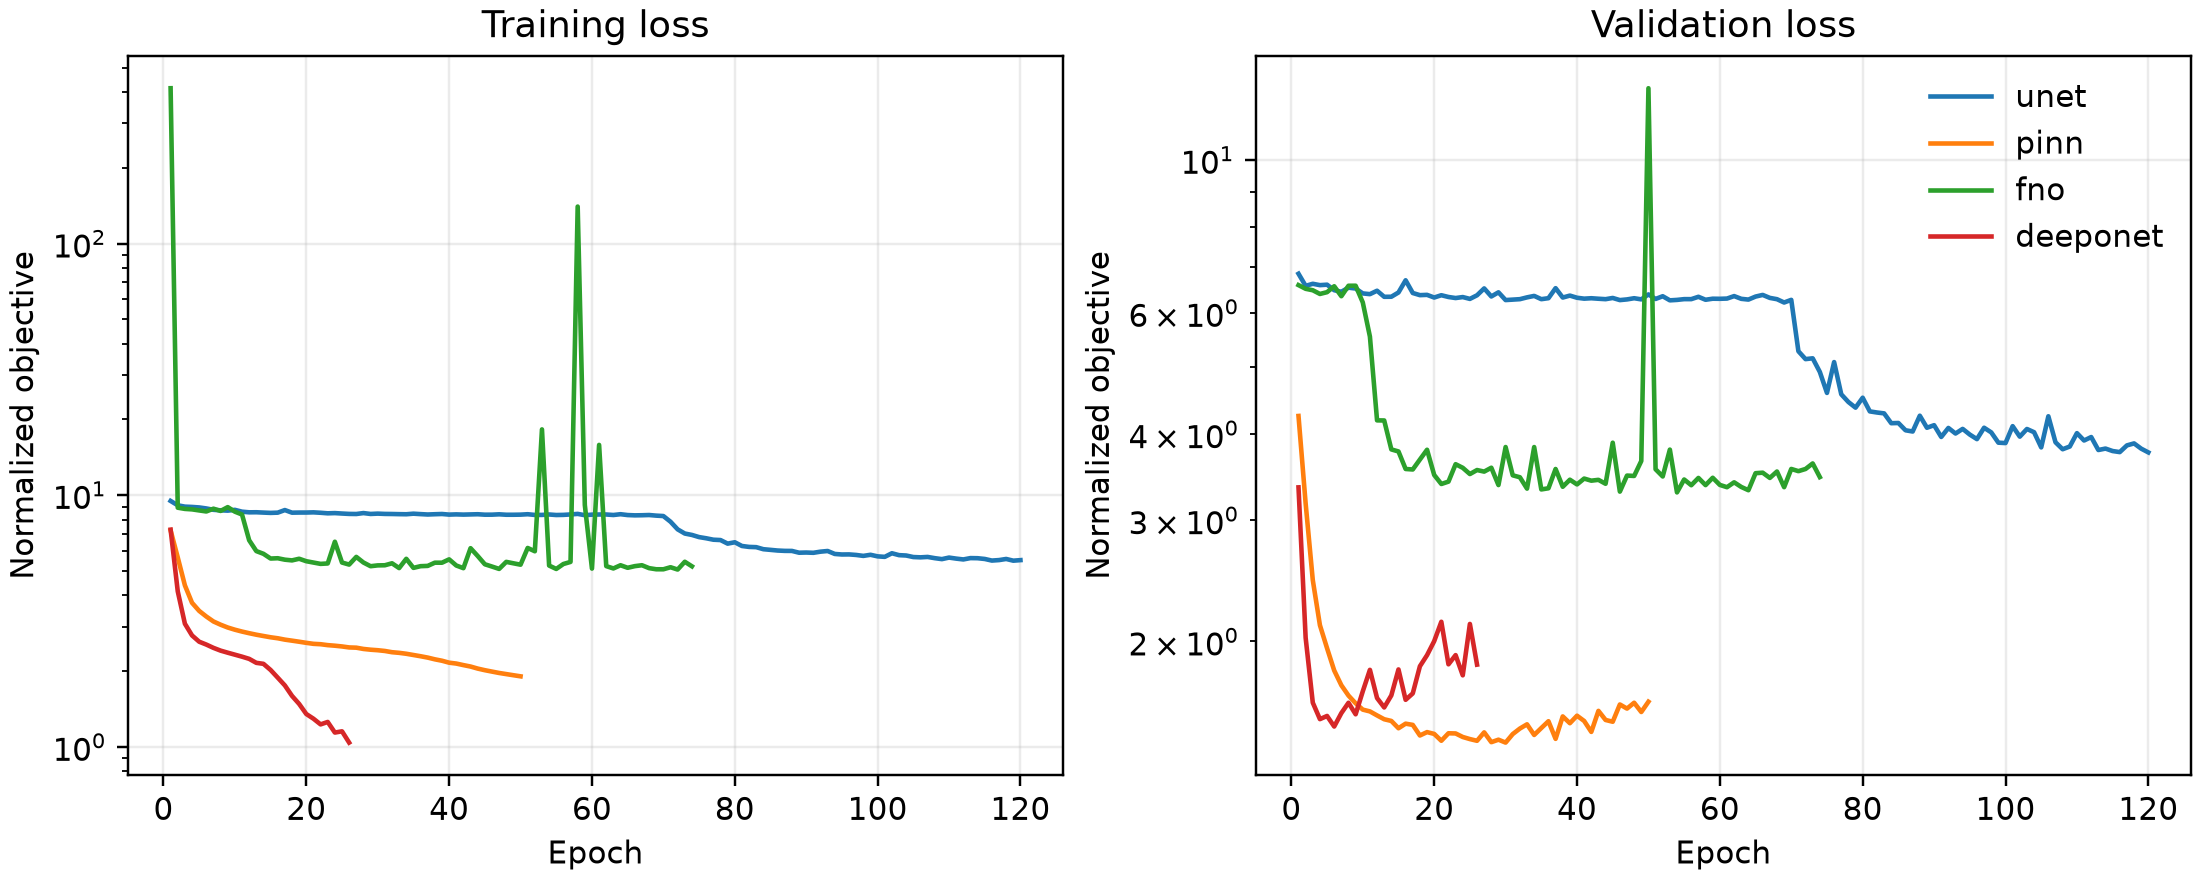
\includegraphics[width=0.83\textwidth]{figures/training_loss_curves.png}
\caption{Training and unseen-geometry validation objectives. Curves terminate
after early stopping; objectives combine normalized field and force losses.}
\label{fig:training}
\end{figure*}

Although surface-pressure integration was implemented as a diagnostic, the coarse common grid did not reproduce absolute OpenFOAM forces reliably because it omits viscous traction and under-resolves the wall. Therefore, optimization uses dedicated $C_L$ and $C_D$ output heads trained on OpenFOAM's total force coefficients. This choice avoids presenting an invalid pressure-only force calculator as ground truth, but it also means force prediction is directly supervised.

\subsection{Common optimization protocol}
At $Re=5\times10^5$, every model optimizes the NACA variables $\theta=(m,p,t,\alpha)$ from NACA 0012, 2412, and 4415 starts. Bounds are $m\in[0,0.09]$, $p\in[0.1,0.9]$, $t\in[0.06,0.20]$, and $\alpha\in[-4,10]^{\circ}$. Nelder--Mead \cite{nelder1965simplex} runs for at most 40 iterations with identical tolerances. The objective is
\begin{equation}
J(\theta)=\frac{C_L}{|C_D|+10^{-6}}-10P_M-5f_M,
\end{equation}
where $P_M$ penalizes a predicted minimum cavitation margin below 5000~Pa and $f_M$ is the fraction of cells below that margin. At the nominal ambient pressure, all selected designs remain far above the threshold, so the cavitation penalty is inactive; the separate ambient-pressure sweep evaluates inception classification under reduced pressure. For each architecture, we select the highest-scoring design across starts and create a new mesh and OpenFOAM case without using surrogate predictions to initialize the solver.

\section{Results}
\subsection{Validation accuracy and computational cost}
Table~\ref{tab:performance} reports results on the 64-case validation set. The physics-regularized network is best for pressure and $C_p$, with a pressure RMSE of 6.78~Pa and $R^2=0.966$. DeepONet gives the best $U_x$, $U_y$, $C_L$, and $C_D$ coefficients. The grid operators are weaker in this low-data setting. FNO retains useful force trends. CNN-U-Net predicts $C_p$ and forces more accurately than absolute pressure or streamwise velocity. The normalized multi-target loss and the affine relationship between $p$ and $C_p$ allow this difference between channels.

\begin{table}[t]
\caption{Validation performance, model size, and cost. Force RMSE is computed case-wise against OpenFOAM total coefficients.}
\label{tab:performance}
\centering
\resizebox{\columnwidth}{!}{%
\begin{tabular}{lrrrrrr}
\toprule
Model & $p$ RMSE & $p$ $R^2$ & $C_L$ RMSE & $C_D$ RMSE & Params. & Speedup \\
\midrule
CNN-U-Net & 28.52 & 0.392 & 0.0991 & 0.00453 & 485,178 & 1,148$\times$ \\
Physics-reg. MLP & \textbf{6.78} & \textbf{0.966} & \textbf{0.0245} & 0.00204 & \textbf{9,930} & \textbf{1,801$\times$} \\
FNO & 22.73 & 0.614 & 0.1383 & 0.00957 & 595,914 & 1,028$\times$ \\
DeepONet & 8.55 & 0.945 & 0.0268 & \textbf{0.00184} & 100,746 & 917$\times$ \\
\bottomrule
\end{tabular}}
\end{table}

Measured training times are 868, 104, 547, and 54~s for CNN-U-Net, the physics-regularized network, FNO, and DeepONet, respectively. Median OpenFOAM execution time is 12.4~s per case, while pressure-field inference requires 0.0069--0.0135~s, yielding 917--1801$\times$ speedups. The benchmark used an 8-core Apple M2 Mac mini with 16~GB memory; PyTorch 2.13 ran on CPU and single-process OpenFOAM 9 ran in Docker. These numbers measure repeated local inference and exclude data generation and mesh construction.

\begin{figure}[t]
\centering
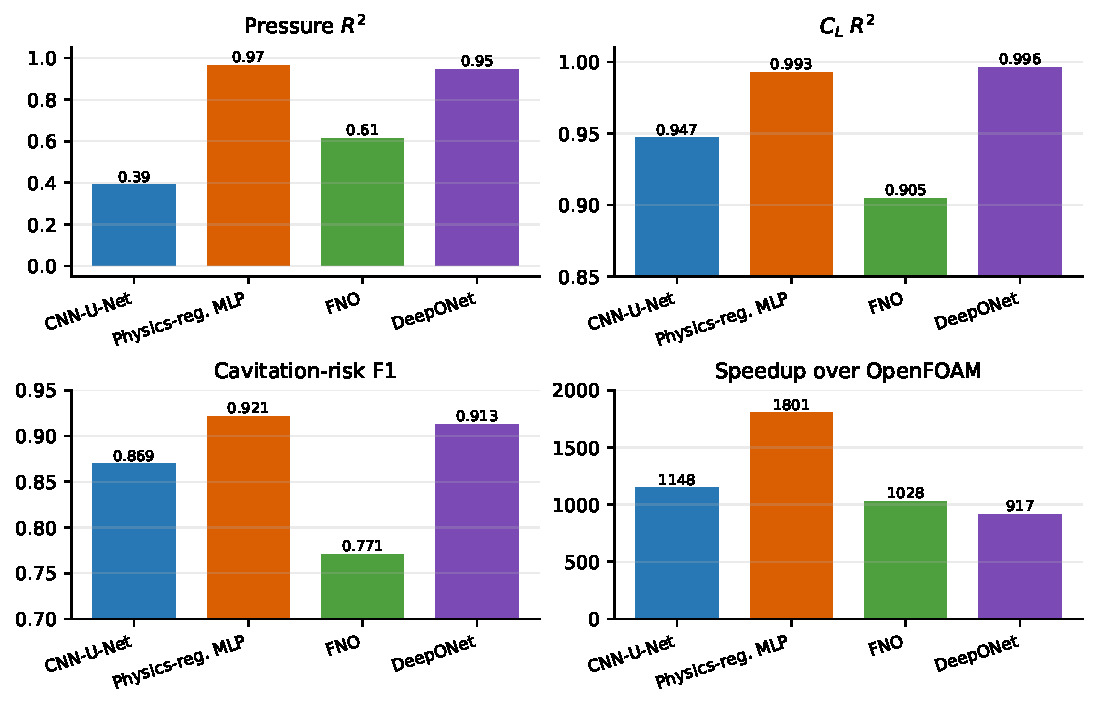
\includegraphics[width=\columnwidth]{figures/model_tradeoffs.pdf}
\caption{No architecture dominates every criterion on the 64-case validation set. Cavitation F1 is aggregated over ambient-pressure sweeps.}
\label{fig:tradeoff}
\end{figure}

Figure~\ref{fig:pressure} shows a representative validation case from the unseen NACA 0015 family. The
pointwise models reproduce the leading-edge pressure structure most closely;
CNN-U-Net smooths the extrema and FNO introduces spatial texture. The distinct
error color scales in the lower row are retained to expose each model's error
structure rather than visually equalizing models with very different ranges.

\begin{figure*}[t]
\centering
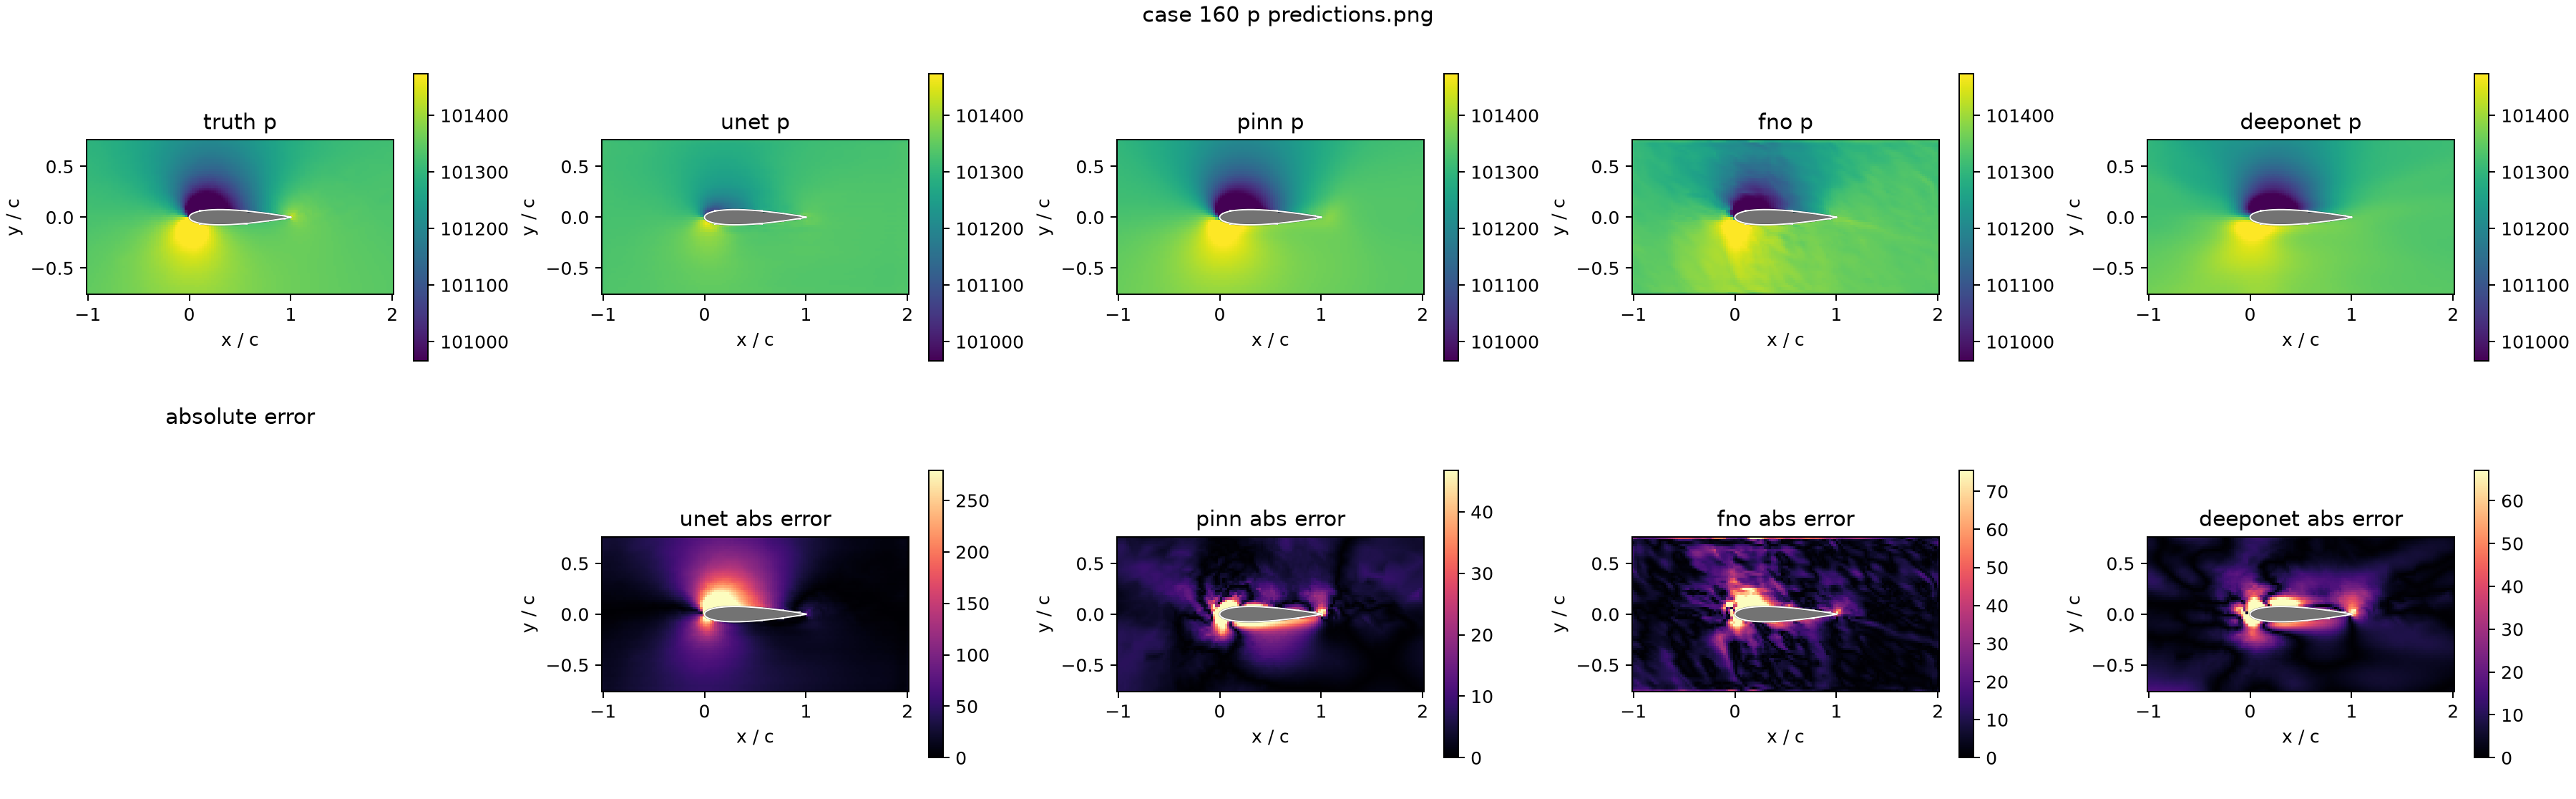
\includegraphics[width=0.97\textwidth]{figures/heldout_pressure.png}
\caption{Absolute-pressure prediction for a representative validation case from the NACA 0015
case (case 160), followed by per-model absolute error. All prediction panels
share the truth color scale; error panels use individually labeled scales.}
\label{fig:pressure}
\end{figure*}

\subsection{Cavitation-inception screening}
The pressure-threshold labels are highly imbalanced, so accuracy is not useful here. The physics-regularized network achieves precision 0.927, recall 0.916, and F1 0.921. DeepONet follows at F1 0.913. CNN-U-Net has the highest recall (0.958) but lower precision (0.796), while FNO obtains F1 0.771. Twenty-four validation case/ambient-pressure combinations contain at-risk cells. This test measures whether a surrogate preserves low-$C_p$ regions well enough for inception screening. It does not model cavity dynamics. That would require multiphase RANS labels such as vapor volume fraction and cavity length \cite{brennen1995cavitation}.

\subsection{CFD-revalidated optimization}
Table~\ref{tab:optimization} and Fig.~\ref{fig:optimization} compare each model's predicted winner with a fresh OpenFOAM solve. All four winners improve upon their associated starting foil in CFD, but by very different amounts. The physics-regularized network selects a thin, strongly cambered profile whose validated $L/D=45.96$ is 79.7\% above the NACA 4415 baseline. DeepONet obtains a 57.8\% improvement and CNN-U-Net obtains 48.5\%. FNO predicts the lowest-performing winner; revalidation gives only a 2.3\% gain over its baseline.

\begin{table}[t]
\caption{Surrogate-selected winners and independent OpenFOAM revalidation. Improvement is relative to the corresponding start at the optimization condition.}
\label{tab:optimization}
\centering
\resizebox{\columnwidth}{!}{%
\begin{tabular}{lrrrrr}
\toprule
Model & Start & Pred. $L/D$ & CFD $L/D$ & Error & CFD gain \\
\midrule
CNN-U-Net & 2412 & 30.17 & 38.45 & $-21.5\%$ & 48.5\% \\
Physics-reg. MLP & 4415 & 43.62 & 45.96 & $-5.1\%$ & \textbf{79.7\%} \\
FNO & 4415 & 21.11 & 26.15 & $-19.3\%$ & 2.3\% \\
DeepONet & 2412 & 39.99 & 40.86 & $-2.1\%$ & 57.8\% \\
\bottomrule
\end{tabular}}
\end{table}

\begin{figure}[t]
\centering
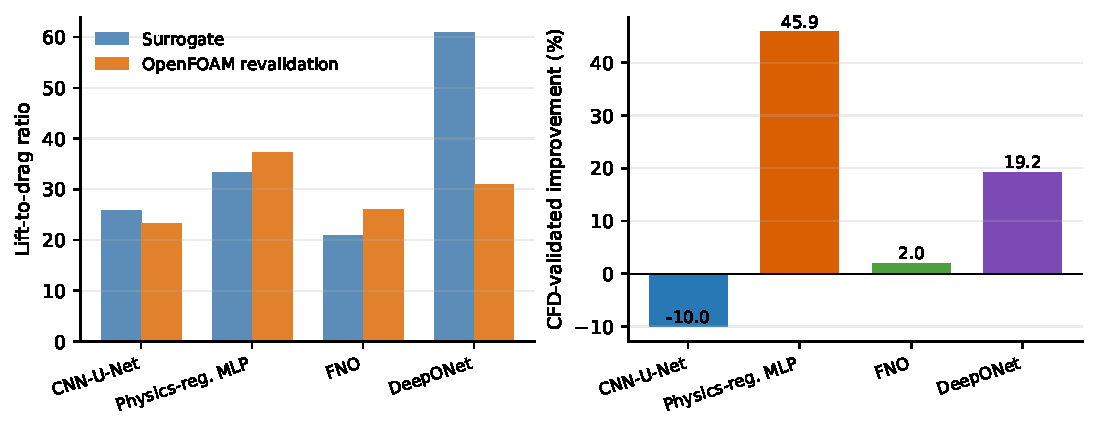
\includegraphics[width=\columnwidth]{figures/optimization_validation.pdf}
\caption{Predicted and OpenFOAM-revalidated performance of each surrogate's selected design. Error in absolute $L/D$ does not by itself determine whether a useful improvement is found.}
\label{fig:optimization}
\end{figure}

The optimization test sharpens the field benchmark in two ways. First, DeepONet gives the smallest winner-level $L/D$ discrepancy, consistent with its force accuracy, but the physics-regularized model finds the best validated design. Second, the FNO winner improves after CFD revalidation yet remains close to its baseline, showing that a conservative prediction error does not guarantee strong search guidance. Screening of five randomly perturbed profiles and an oval was also performed, but these geometries lie outside the NACA training manifold and are reported only as stress tests, not validated free-form design evidence.

\section{Scope and Next Steps}
The pointwise models outperform the grid operators in this low-data, fixed-grid experiment. The result is useful precisely because all four models see the same cases, targets, split, and optimization task. It is not a universal ranking. Larger operator-learning datasets or different loss balancing may favor CNN-U-Net or FNO.

Pressure accuracy, force accuracy, and optimization quality capture different parts of the workflow. DeepONet is the most accurate force model, while the physics-regularized network returns the best CFD-validated design. The optimizer concentrates queries in a small region and can amplify structured prediction error. For that reason, a CFD solve remains the final step in the design loop.

The current scope is two-dimensional, steady, single-phase RANS over NACA four-digit profiles. Three divergent force cases are removed by a fixed quality rule. A symmetry audit also finds a small lift bias at zero incidence. The study does not yet include grid-convergence or turbulence-model sensitivity, and the validation families do not represent arbitrary topology. Force coefficients are directly supervised because the common grid cannot resolve pressure and viscous traction accurately enough for force integration. We rerun one winner per model. Cavitation is evaluated as pressure-threshold inception risk, not vapor transport or unsteady shedding.

The next steps are repeated training seeds, mesh and turbulence sensitivity, more CFD checks around each optimum, uncertainty-guided sampling, and multiphase or experimental cavitation labels. These extensions broaden the claim; they do not change the present benchmark result that architecture choice affects both prediction accuracy and the design returned by the optimizer.

\subsection{Practical model selection}
The timing results are most useful when interpreted as amortized workflow costs.
Dividing each measured training time by the per-case time saved relative to
OpenFOAM gives approximate break-even points of 70 new evaluations for
CNN-U-Net, 8 for the physics-regularized network, 44 for FNO, and 5 for
DeepONet. These values exclude the CFD corpus, which is a shared prerequisite
for all four supervised models, but they show that training cost is recovered
quickly once a model is used for optimization or a broad operating sweep. The
physics-regularized model is especially favorable here: its parameter count is
roughly 1/49 that of CNN-U-Net and 1/60 that of FNO, yet it has the fastest
inference and strongest validated design result.

Speed alone, however, is not an adequate deployment rule. A practical workflow
can separate three roles. First, a fast surrogate screens thousands of candidate
operating points or geometries. Second, a verification policy sends selected
candidates back to CFD based on predicted merit, model disagreement, distance
from the training manifold, or uncertainty. Third, verified cases are appended
to the training set before another optimization round. The present experiment
implements the first role and a fixed version of the second by revalidating one
winner per architecture. It does not yet adaptively retrain. The disagreement
between FNO's search outcome and those of the pointwise models suggests that
cross-model consensus could already serve as a simple warning signal: a design
preferred only by the weakest model on the validation set deserves a larger
verification budget than one supported by several independently structured
surrogates.

Architecture selection should therefore follow the intended scientific action.
DeepONet is attractive when accurate force coefficients and faithful ranking are
primary. The physics-regularized network is the strongest choice in this low-data
study when pressure, inception screening, runtime, and final design improvement
are considered jointly. CNN-U-Net's high inception recall may be useful for
conservative screening, despite its poorer pressure field, while the current FNO
requires more data or tuning before design deployment. This task-specific view is
more actionable than naming a single winner from an averaged multi-output loss.

\subsection{Reproducibility and evidence boundaries}
The benchmark was built around machine-readable provenance rather than a single
summary spreadsheet. Each processed case retains its operating parameters,
geometry descriptors, source identifier, fluid mask, signed distance, field
targets, and OpenFOAM force coefficients. The deterministic split is regenerated
from the valid case list and seed, while every checkpoint stores its target and
input field order, normalization, architecture arguments, and training history.
Evaluation scripts write per-case CSV files before producing aggregate metrics.
Similarly, optimization records every parameter vector and objective evaluation,
and the four revalidation directories contain the generated meshes, solver logs,
final fields, and force histories. This structure permits headline values to be
traced from a table back to the underlying case rather than reconstructed from a
plot.

The audit also records exclusions and failed checks. Exact cross-angle pressure duplicates
are absent in the corrected dataset, three nonphysical force cases are excluded
by a predeclared $|C|\leq5$ rule, and random or oval profiles are marked as
tests outside the training geometry family. We report the small symmetric-foil lift bias
rather than using symmetry as an assumed validation. For runtime, the scripts
parse OpenFOAM's logged execution time and time pressure-field inference over the
same selected cases; they do not fold the one-time training cost into the speedup.
For cavitation, the evaluation artifact labels every result as pressure-threshold
inception risk. These boundaries are part of the result: an auditable scientific
ML workflow should preserve not only successful metrics but also exclusions,
inactive constraints, and conditions under which a claim ceases to apply.

\section{Conclusion}
We benchmarked four neural surrogates for hydrofoil RANS prediction, cavitation-risk screening, and shape optimization. The physics-regularized network gives the best pressure accuracy, inception-risk F1, speed, and CFD-validated design improvement. DeepONet predicts force coefficients most accurately. CNN-U-Net remains competitive for $C_p$, force prediction, and high-recall risk screening, while FNO is weaker in this low-data setting. All models are 917--1801$\times$ faster than the measured OpenFOAM solves. The optimization results show why a useful surrogate benchmark should include both validation accuracy and CFD checks of the designs the models select.

\section*{Artifact Availability}
Code, configurations, split definitions, trained checkpoints, per-case metrics, optimization traces, and OpenFOAM validation cases are organized in an auditable repository. An anonymized archival link will be added before submission.

\IEEEtriggeratref{6}
\bibliographystyle{IEEEtran}
\bibliography{references}

\end{document}
